
\section{Desigualdades clássicas}
\begin{frame}
\frametitle{Desigualdades clássicas} 

Para iniciar, apresentamos algumas desigualdades simples mas
famosas, válidas para quaisquer $a,b \in \R$:
\begin{itemize}
	\item $\modu a \geq 0$;
	\item $a^2 \geq 0$;
	\item $\modu {a+b} \leq \modu a + \modu b$ (desigualdade triangular).
\end{itemize}

\end{frame}
%------------------------------------------------------------------------------------------------------------
\begin{frame}
\frametitle{Desigualdades clássicas} 

\begin{teorema}[Desigualdade Triangular]
	Dado um triângulo $ABC$ como o abaixo,
	\label{fig:destri1}
	\begin{figure}[H]
	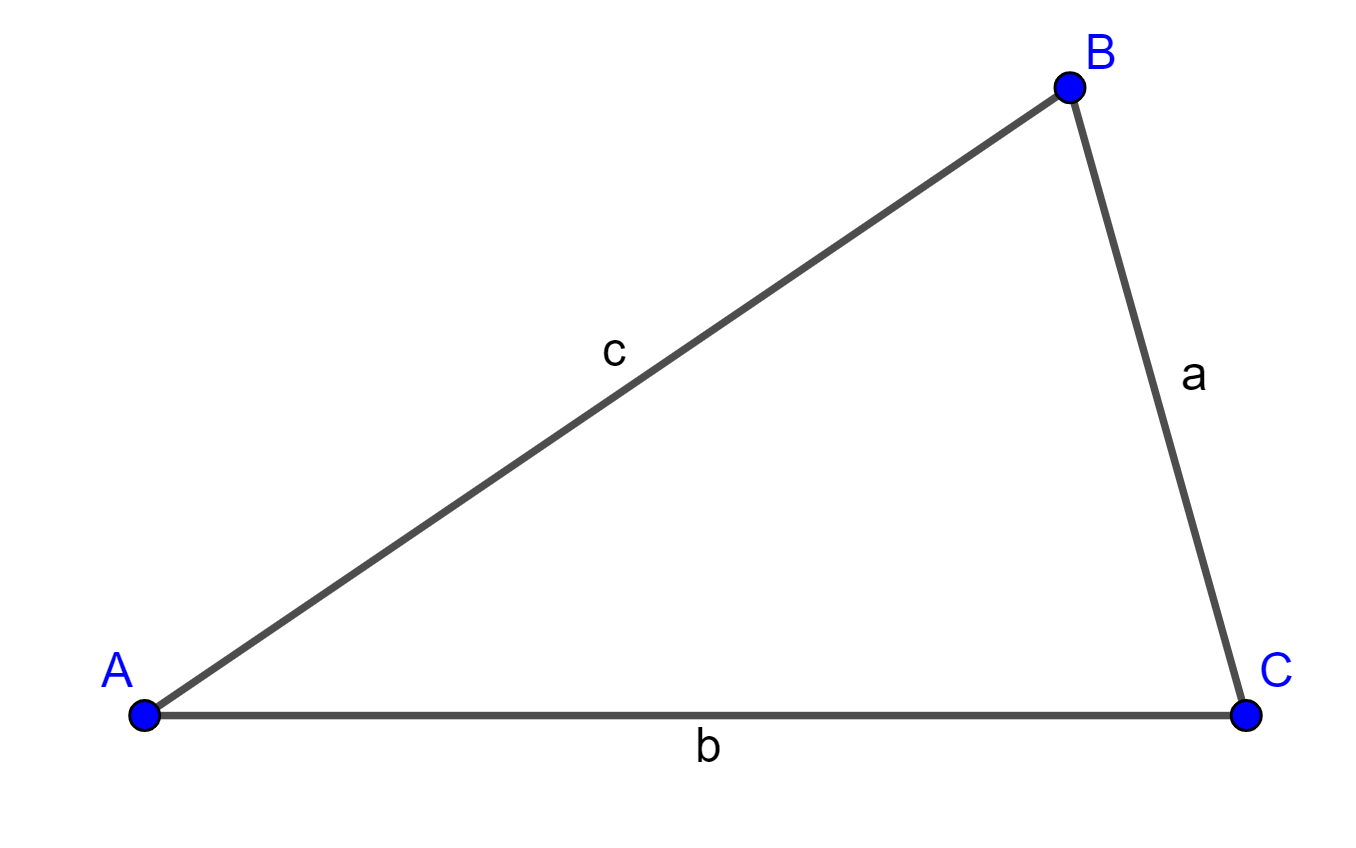
\includegraphics[scale=0.24]{figures/DesTriang1.png}
	\centering
	\end{figure}
	o comprimento de um dos lados é sempre inferior à soma dos comprimentos dos outros dois lados, ou seja, $a< b+c$, $b<a+c$ e $c< a+b$. A igualdade $a = b+c$ ocorre se, e somente se, os pontos $A$, $B$ e $C$ forem colineares e $A$ estiver entre $B$ e $C$.
\end{teorema}

\end{frame}
%------------------------------------------------------------------------------------------------------------
